\documentclass[12pt,letterpaper]{article}
\usepackage[a4paper, top=1.2in, bottom=1.4in, left=1in, right=1in]{geometry}
\usepackage{graphicx} % Required for inserting images
\graphicspath{ {./img/} }
\usepackage[spanish]{babel}
\usepackage{float}
\usepackage{fancyhdr}
\setlength{\parskip}{1em}  % Adds space between paragraphs (1em)
\usepackage{amsmath,amssymb}
\usepackage{booktabs}
\usepackage{tikz}
\usepackage{listings}
\usepackage[utf8]{inputenc}

\usepackage{xcolor}

\lstset{
    language=Python,
    basicstyle=\ttfamily\footnotesize,
    keywordstyle=\color{blue}\bfseries,
    commentstyle=\color{gray}\itshape,
    stringstyle=\color{orange},
    showstringspaces=false,
    frame=single,
    breaklines=true
}
\usepackage{subcaption}
\newcommand{\tikzmark}[1]{\tikz[baseline,remember picture] \coordinate (#1) {};}
\usetikzlibrary{positioning}
\usetikzlibrary{shadows,arrows.meta} % For adding edges label
\usetikzlibrary{calc}
\usepackage{eso-pic}
\usepackage[backend=biber, defernumbers=true, citestyle=numeric-comp, bibstyle=ieee, sorting=none]{biblatex}
\addbibresource{bibliography/bibliography.bib}
\DeclareBibliographyCategory{cited}
\AtEveryCitekey{\addtocategory{cited}{\thefield{entrykey}}}
% Configurando BibLaTeX
\DefineBibliographyStrings{spanish}{
  url = {URL},
  andothers={et ~al\adddot}
}
\usepackage{listings}
\usepackage{xcolor}

\definecolor{codegreen}{rgb}{0,0.6,0}
\definecolor{codegray}{rgb}{0.5,0.5,0.5}
\definecolor{codepurple}{rgb}{0.58,0,0.82}
\definecolor{backcolour}{rgb}{0.95,0.95,0.92}

\lstdefinestyle{mystyle}{
    backgroundcolor=\color{backcolour},   
    commentstyle=\color{codegreen},
    keywordstyle=\color{magenta},
    numberstyle=\tiny\color{codegray},
    stringstyle=\color{codepurple},
    basicstyle=\ttfamily\footnotesize,
    breakatwhitespace=false,         
    breaklines=true,                 
    captionpos=b,                    
    keepspaces=true,                 
    numbers=left,                    
    numbersep=5pt,                  
    showspaces=false,                
    showstringspaces=false,
    showtabs=false,                  
    tabsize=2
}

\lstset{style=mystyle}

\AddToShipoutPictureBG{%
\begin{tikzpicture}[remember picture, overlay]
\node[opacity=.15, inner sep=0pt]
    at(current page.center){
\includegraphics[scale=1.5]{img/logo-ugr2.png}};
\end{tikzpicture}%
}

\title{Agente conversacional potenciado por RAG}
\author{Miguel García López}
\date{Mayo 2025}

\pagestyle{fancyplain}
\headheight 35pt
\lhead{Miguel García López}            
\chead{\textbf{\small RAG-Agent}}
\rhead{SRIR \\ \today}
\lfoot{\scriptsize\LaTeX}
\cfoot{\small Agente conversacional potenciado por RAG}
\rfoot{\small\thepage}
\headsep 1.5em

\author{Miguel García López} % Nombre y apellidos

\date{\normalsize\today} % Incluye la fecha actual

\begin{document}
\begin{titlepage}
    \begin{figure}
        \vspace{-1.3cm}
        \begin{center}
            
\includegraphics[width=0.75\textwidth]{img/UGR-Logo.png}
        \end{center}
    \end{figure}
    \vspace{1.3cm}
    \centering
    \normalfont \normalsize
    \textsc{\textbf{Sistemas de Recuperación de Información y de Recomendación - 2024-2025} \\\vspace{.15cm} Universidad de Granada} \\ [25pt]
    \huge Agente potenciado por sistema RAG

    \normalfont \normalsize \vspace{.30cm}
    \textsc{Miguel García López}

\end{titlepage}

\tableofcontents
\listoffigures
\listoftables
\newpage

\section{Objetivos}
Este documento tiene como objetivo principal explicar de forma clara y suficientemente detallada la implementación de un agente conversacional potenciado con un sistema \textit{RAG} (\textit{Retrieval-Augmented Generation}).

Se procederá a una explicación detallada del proceso de diseño, así como tecnologías usadas, patrones de diseño de clases y tipos de métodos usados.

También se explicarán ciertos conceptos teóricos, como qué es un agente y qué es un \textit{RAG}.

\section{Introducción}
En este trabajo se detallan y explican los procesos llevados a cabo en la creación de un agente conversacional potenciado con un sistema \textit{RAG}, que es fundamentalmente, un sistema muy potente de recuperación de información.

Este tipo de técnicas han sido usadas desde hace muchos años atrás en el tiempo. Antes de la invención formal de los sistemas \textit{RAG} (\textit{Retrieval-Augmented Generation}), existieron numerosos sistemas y enfoques que sentaron las bases conceptuales para esta tecnología. Por ejemplo, en \cite{salton1983introduction} se establecieron las bases de los sistemas modernos de recuperación de información, introduciendo conceptos como el modelo de espacio vectorial que más tarde serían fundamentales para \textit{RAG}.

\section{Tecnologías Utilizadas}

El sistema conversacional con capacidades \textit{RAG} desarrollado en este trabajo se apoya en un conjunto de tecnologías avanzadas en inteligencia artificial y procesamiento de lenguaje natural. Para la recuperación eficiente de información se utiliza \textit{FAISS} \cite{johnson2019billion}, mientras que \textit{Sentence-Transformers} permite generar representaciones semánticas de consultas y documentos. La generación de respuestas se basa en los modelos de lenguaje de \textit{OpenAI}, integrados mediante técnicas de \textit{prompt engineering}. \textit{LangGraph} facilita la orquestación de los componentes mediante estructuras de flujo conversacional. \textit{NumPy} se encarga del manejo eficiente de datos vectoriales, y \textit{Streamlit} proporciona una interfaz web interactiva que permite al usuario visualizar y entender el funcionamiento del sistema.


\section{Teoría}

En esta sección se presentan los fundamentos teóricos de las dos tecnologías principales empleadas en este trabajo: los sistemas de Generación Aumentada por Recuperación (\textit{RAG}) y los agentes basados en modelos de lenguaje. Ambos representan avances significativos en el campo de la inteligencia artificial aplicada al procesamiento del lenguaje natural y la creación de sistemas conversacionales inteligentes.

\subsection{Generación Aumentada por Recuperación (RAG)}

La Generación Aumentada por Recuperación (\textit{Retrieval-Augmented Generation} o \textit{RAG}) \cite{lewis2020retrieval} es un paradigma que combina las capacidades generativas de los modelos de lenguaje de gran escala (\textit{Large Language Models} o \textit{LLMs}) con sistemas de recuperación de información para producir respuestas más precisas, actualizadas y verificables.

\subsubsection{Fundamentos del RAG}

Un sistema RAG opera fundamentalmente en dos fases principales:

\begin{enumerate}
    \item \textbf{Fase de Recuperación (\textit{Retrieval})}: Dada una consulta del usuario, el sistema busca y recupera documentos o fragmentos de información relevantes de una base de conocimiento.

    \item \textbf{Fase de Generación (\textit{Generation})}: Los documentos recuperados se incorporan como contexto adicional al \textit{prompt} del modelo de lenguaje, que luego genera una respuesta basada tanto en su conocimiento parametrizado como en la información recuperada.
\end{enumerate}

Esta arquitectura híbrida resuelve varias limitaciones inherentes a los LLMs puros:

\begin{itemize}
    \item \textbf{Conocimiento estático}: Los modelos de lenguaje tienen conocimientos limitados al período hasta su entrenamiento, mientras que RAG permite acceso a información actualizada.

    \item \textbf{Alucinaciones}: Al anclar la generación en fuentes externas verificables, RAG reduce significativamente la tendencia de los LLMs a generar información incorrecta.

    \item \textbf{Transparencia}: RAG puede proporcionar las fuentes de su información, permitiendo verificar la procedencia de las respuestas.

    \item \textbf{Especialización}: Permite adaptar modelos generales a dominios específicos sin necesidad de reentrenamiento.
\end{itemize}

\subsubsection{Estrategias de Fragmentación (\textit{Chunking})}

Un componente crítico en el diseño de sistemas RAG es la estrategia de fragmentación (\textit{chunking}) de los documentos de la base de conocimiento. Entre las principales estrategias se encuentran:

\begin{itemize}
    \item \textbf{Fragmentación por tamaño fijo}: Divide los documentos en fragmentos de un número determinado de tokens o caracteres. Simple pero puede romper la coherencia del texto.

    \item \textbf{Fragmentación por límites semánticos}: Algoritmos más sofisticados que dividen el texto basándose en cambios temáticos o estructuras semánticas.

    \item \textbf{Fragmentación recursiva (\textit{recursive chunking})}: Crea una jerarquía de fragmentos de diferentes granularidades, permitiendo representaciones multi-nivel del conocimiento.
\end{itemize}

La elección de la estrategia de fragmentación afecta directamente a la calidad de la recuperación, ya que fragmentos demasiado grandes pueden contener información irrelevante, mientras que fragmentos demasiado pequeños pueden perder contexto importante.

\subsubsection{Estrategias de Recuperación (\textit{Retrievers})}

El componente de recuperación (\textit{retriever}) de un sistema \textit{RAG} es el encargado de identificar y seleccionar los fragmentos más relevantes para una consulta dada. Las principales tecnologías incluyen:

\begin{itemize}
    \item \textbf{Recuperación basada en \textit{embeddings} densos}: Utiliza representaciones vectoriales densas del texto para capturar la semántica profunda. Tecnologías como modelos basados en \textit{Sentence-Transformers} generan estas representaciones.

    \item \textbf{Recuperación léxica}: Basada en la coincidencia de términos, usando algoritmos como \textit{BM25} \cite{robertson1995okapi} o \textit{TF-IDF}. Más simple pero eficaz para coincidencias exactas.

    \item \textbf{Recuperación híbrida}: Combina métodos semánticos y léxicos para aprovechar las fortalezas de ambos enfoques, como en arquitecturas de tipo \textit{ColBERT} o \textit{REALM}.

\end{itemize}

\subsection{Agentes}
Un agente basado en modelos de lenguaje puede definirse como un sistema que combina un \textit{LLM} con capacidades de acción mediante herramientas (\textit{tools}), permitiéndole realizar tareas concretas en entornos específicos.

\section{Implementación}

\subsection{Patrones de Diseño}

En la implementación del sistema se han utilizado varios patrones de diseño para garantizar modularidad, escalabilidad y facilidad de mantenimiento:

\begin{itemize}
    \item \textbf{Patrón Estrategia (\textit{Strategy})}: Implementado en el módulo de recuperación para permitir la selección dinámica entre diferentes estrategias de recuperación (\textit{embeddings} densos, léxica o híbrida). Se ha utilizado para modelar distintos tipos de técnicas de \textit{chunking} y de recuperación por similitud.

    \item \textbf{Patrón Singleton}: Utilizado para garantizar una única instancia del componente encargado de gestionar el acceso compartido a los recursos del sistema, asegurando una coordinación coherente entre los módulos. Se ha utilizado en la clase \texttt{VectorDB}, que representa la base de datos vectorial.

\end{itemize}

\subsection{Clases y Componentes}

El sistema se compone de dos bloques principales: los \textbf{Chunkers} (figura \ref{fig:chunker}), encargados de dividir el texto en fragmentos, y los \textbf{Retrievers} (figura \ref{fig:retriever}), responsables de recuperar la información más relevante dado un \textit{input}. Estos dos bloques principales encajan dentro de una clase que modele el comportamiento y funcionalidades principales de una base de datos vectorial, de lo cual se encarga la clase \texttt{VectorDB} (figura \ref{fig:vectordb}).

\subsubsection{Chunkers}

\begin{figure}[htp]
    \centering
    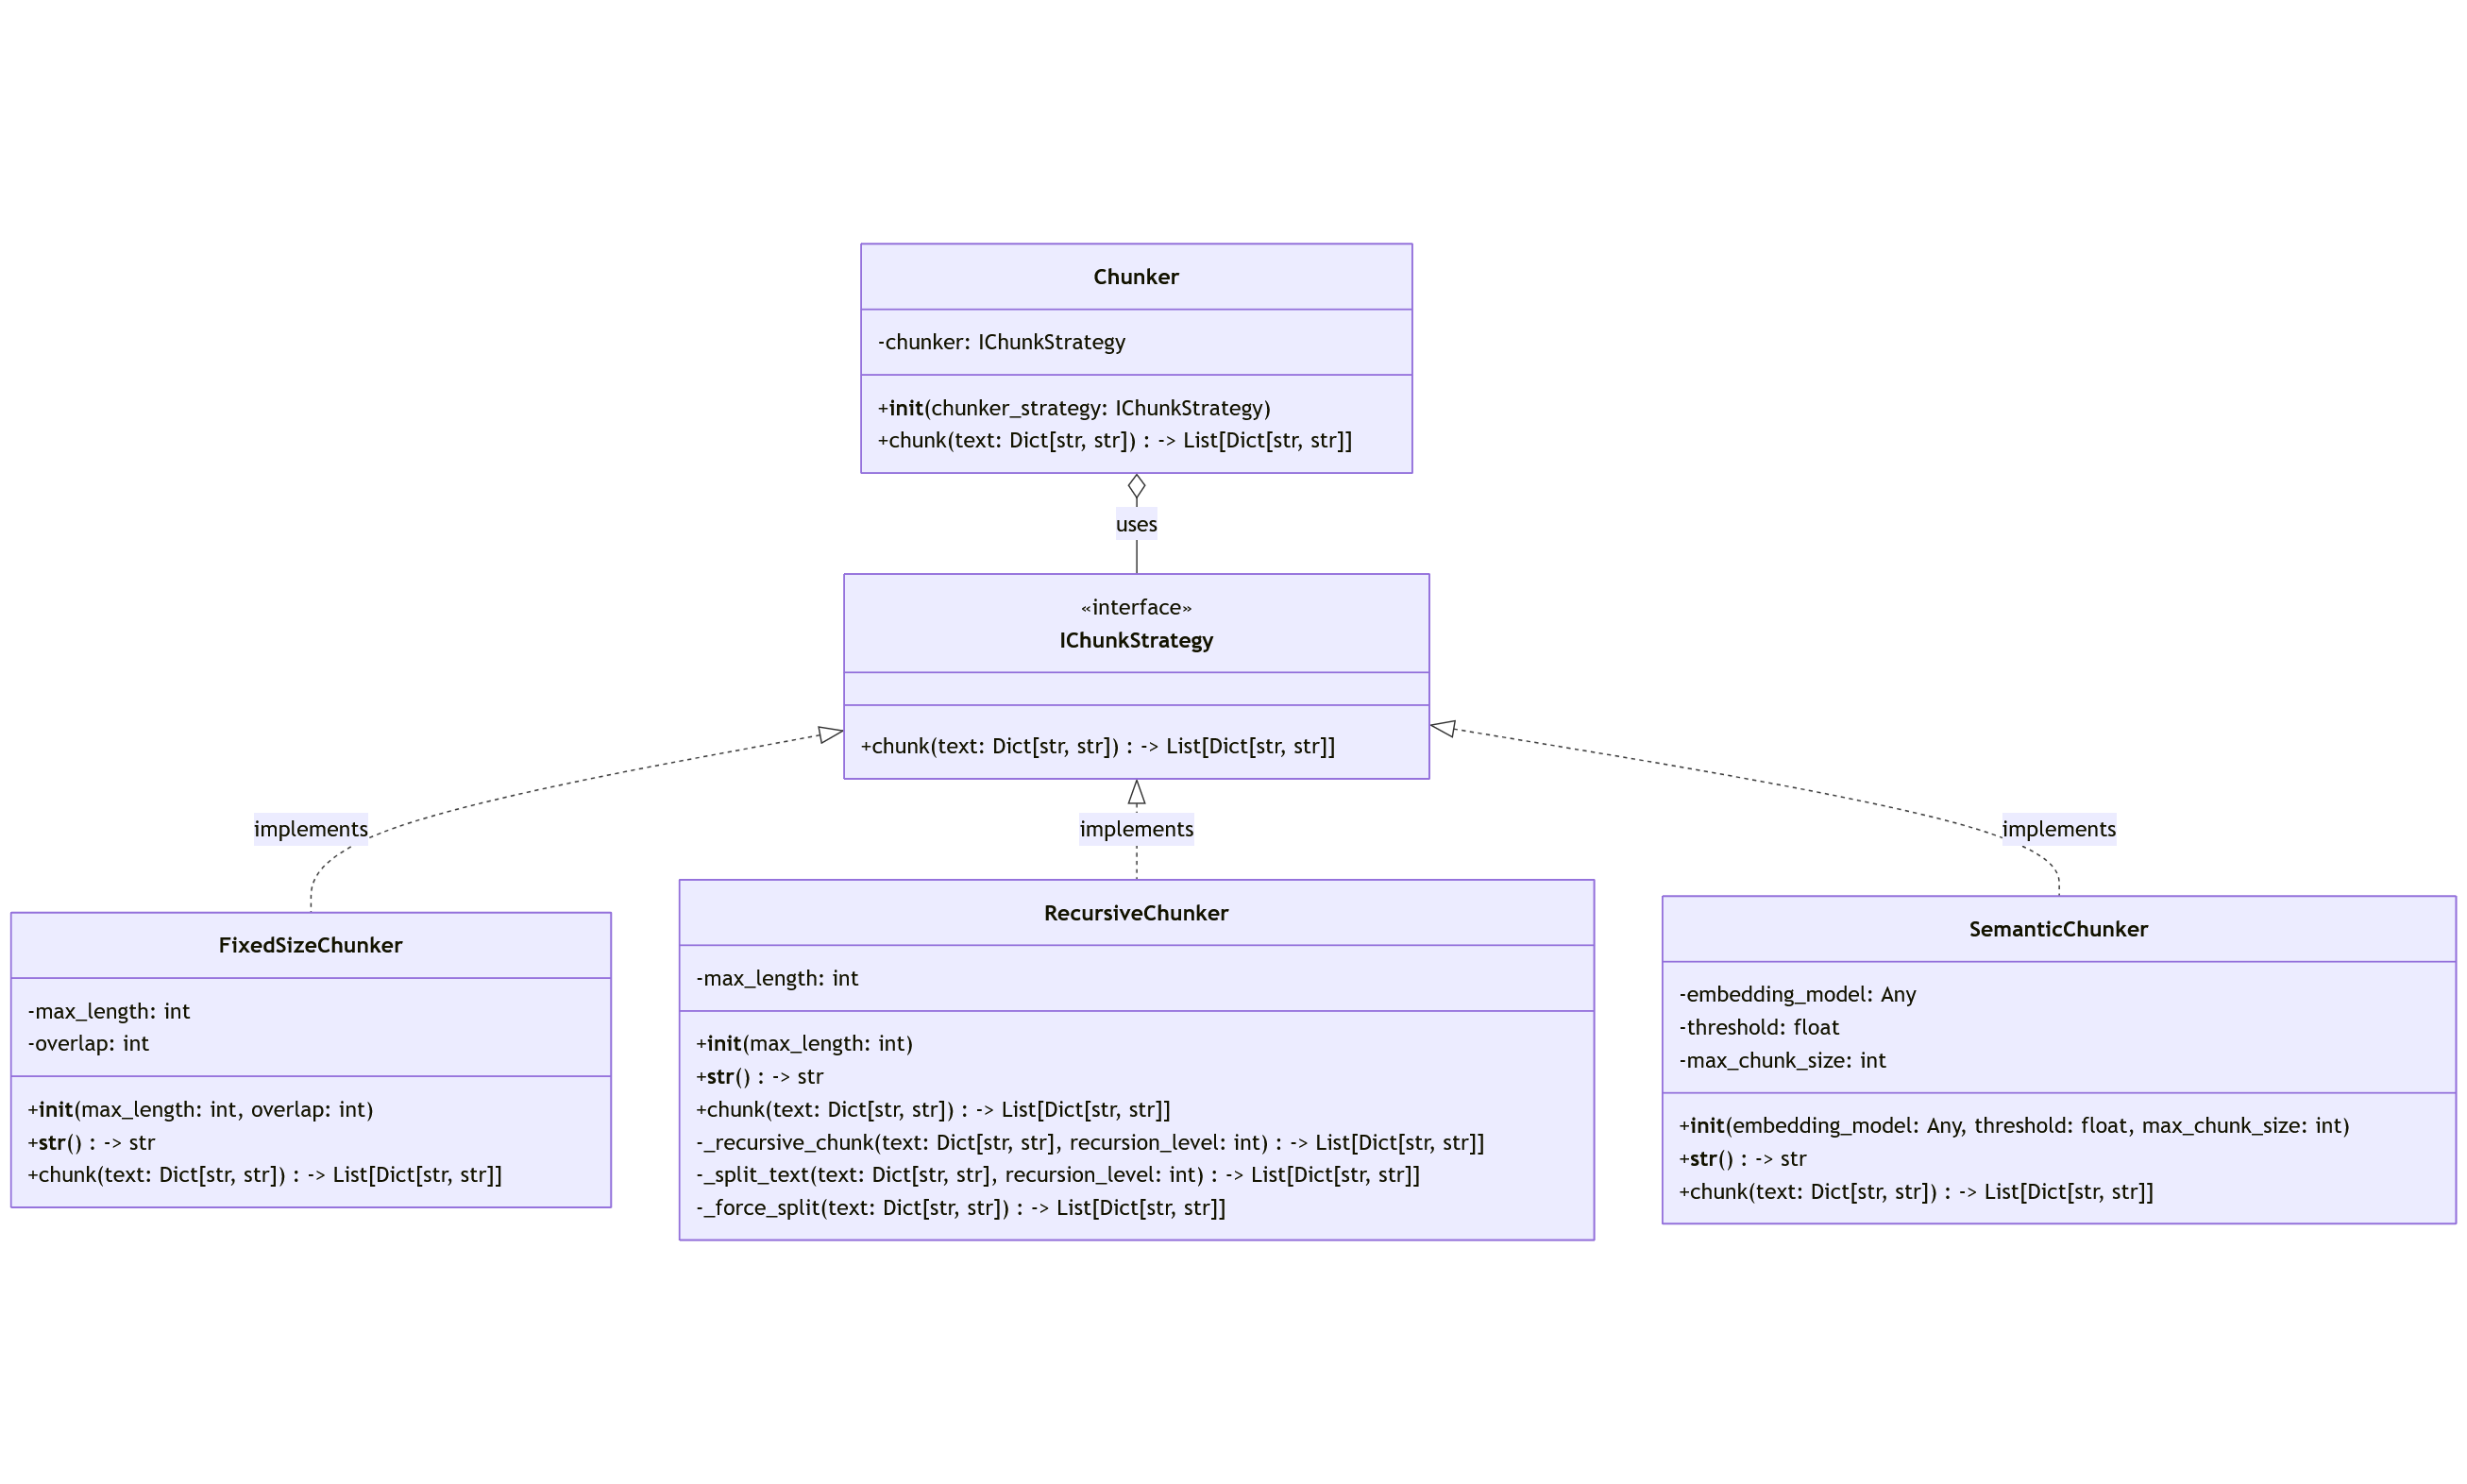
\includegraphics[width=1\linewidth]{img/chunker.png}
    \caption{Diagrama de clase \textit{Chunker}}
    \label{fig:chunker}
\end{figure}

\paragraph{FixedSizeChunker}

Esta clase implementa una estrategia de fragmentación de texto en bloques de longitud fija, permitiendo opcionalmente solapamiento entre ellos.

\begin{itemize}
    \item \textbf{Constructor}: Recibe el tamaño máximo del bloque (\texttt{max\_length}) y un solapamiento opcional (\texttt{overlap}).
    \item \textbf{chunk()}: Divide el texto en fragmentos consecutivos, asegurando que cada fragmento no exceda el tamaño definido y respeta el solapamiento.
\end{itemize}

\paragraph{RecursiveChunker}

Fragmenta el texto de forma jerárquica: por párrafos, luego oraciones, y finalmente palabras, dependiendo del nivel de recursión. Se asegura de que cada fragmento cumpla con una longitud máxima.

\begin{itemize}
    \item \textbf{chunk()}: Llama al método recursivo \texttt{\_recursive\_chunk()}, que adapta el criterio de fragmentación según el nivel de profundidad.
    \item \textbf{\_split\_text()}: Fragmenta el texto por saltos dobles de línea, por oraciones o por palabras, dependiendo del nivel de recursión.
    \item \textbf{\_force\_split()}: En caso de que no se pueda dividir el texto de forma semántica, lo parte en trozos estrictamente según el límite de longitud.
\end{itemize}

\paragraph{SemanticChunker}

Esta clase utiliza \textit{embeddings} para crear fragmentos semánticamente coherentes. Agrupa frases consecutivas en un bloque mientras su similitud coseno permanezca por encima de un umbral definido.

\begin{itemize}
    \item \textbf{Constructor}: Requiere un modelo de \textit{embeddings}, un umbral de similitud y una longitud máxima del fragmento.
    \item \textbf{chunk()}: Calcula los \textit{embeddings} de cada oración y agrupa aquellas cuya similitud sea alta y cuya longitud combinada no exceda el máximo.
\end{itemize}

\subsubsection{Retrievers}

\begin{figure}[htp]
    \centering
    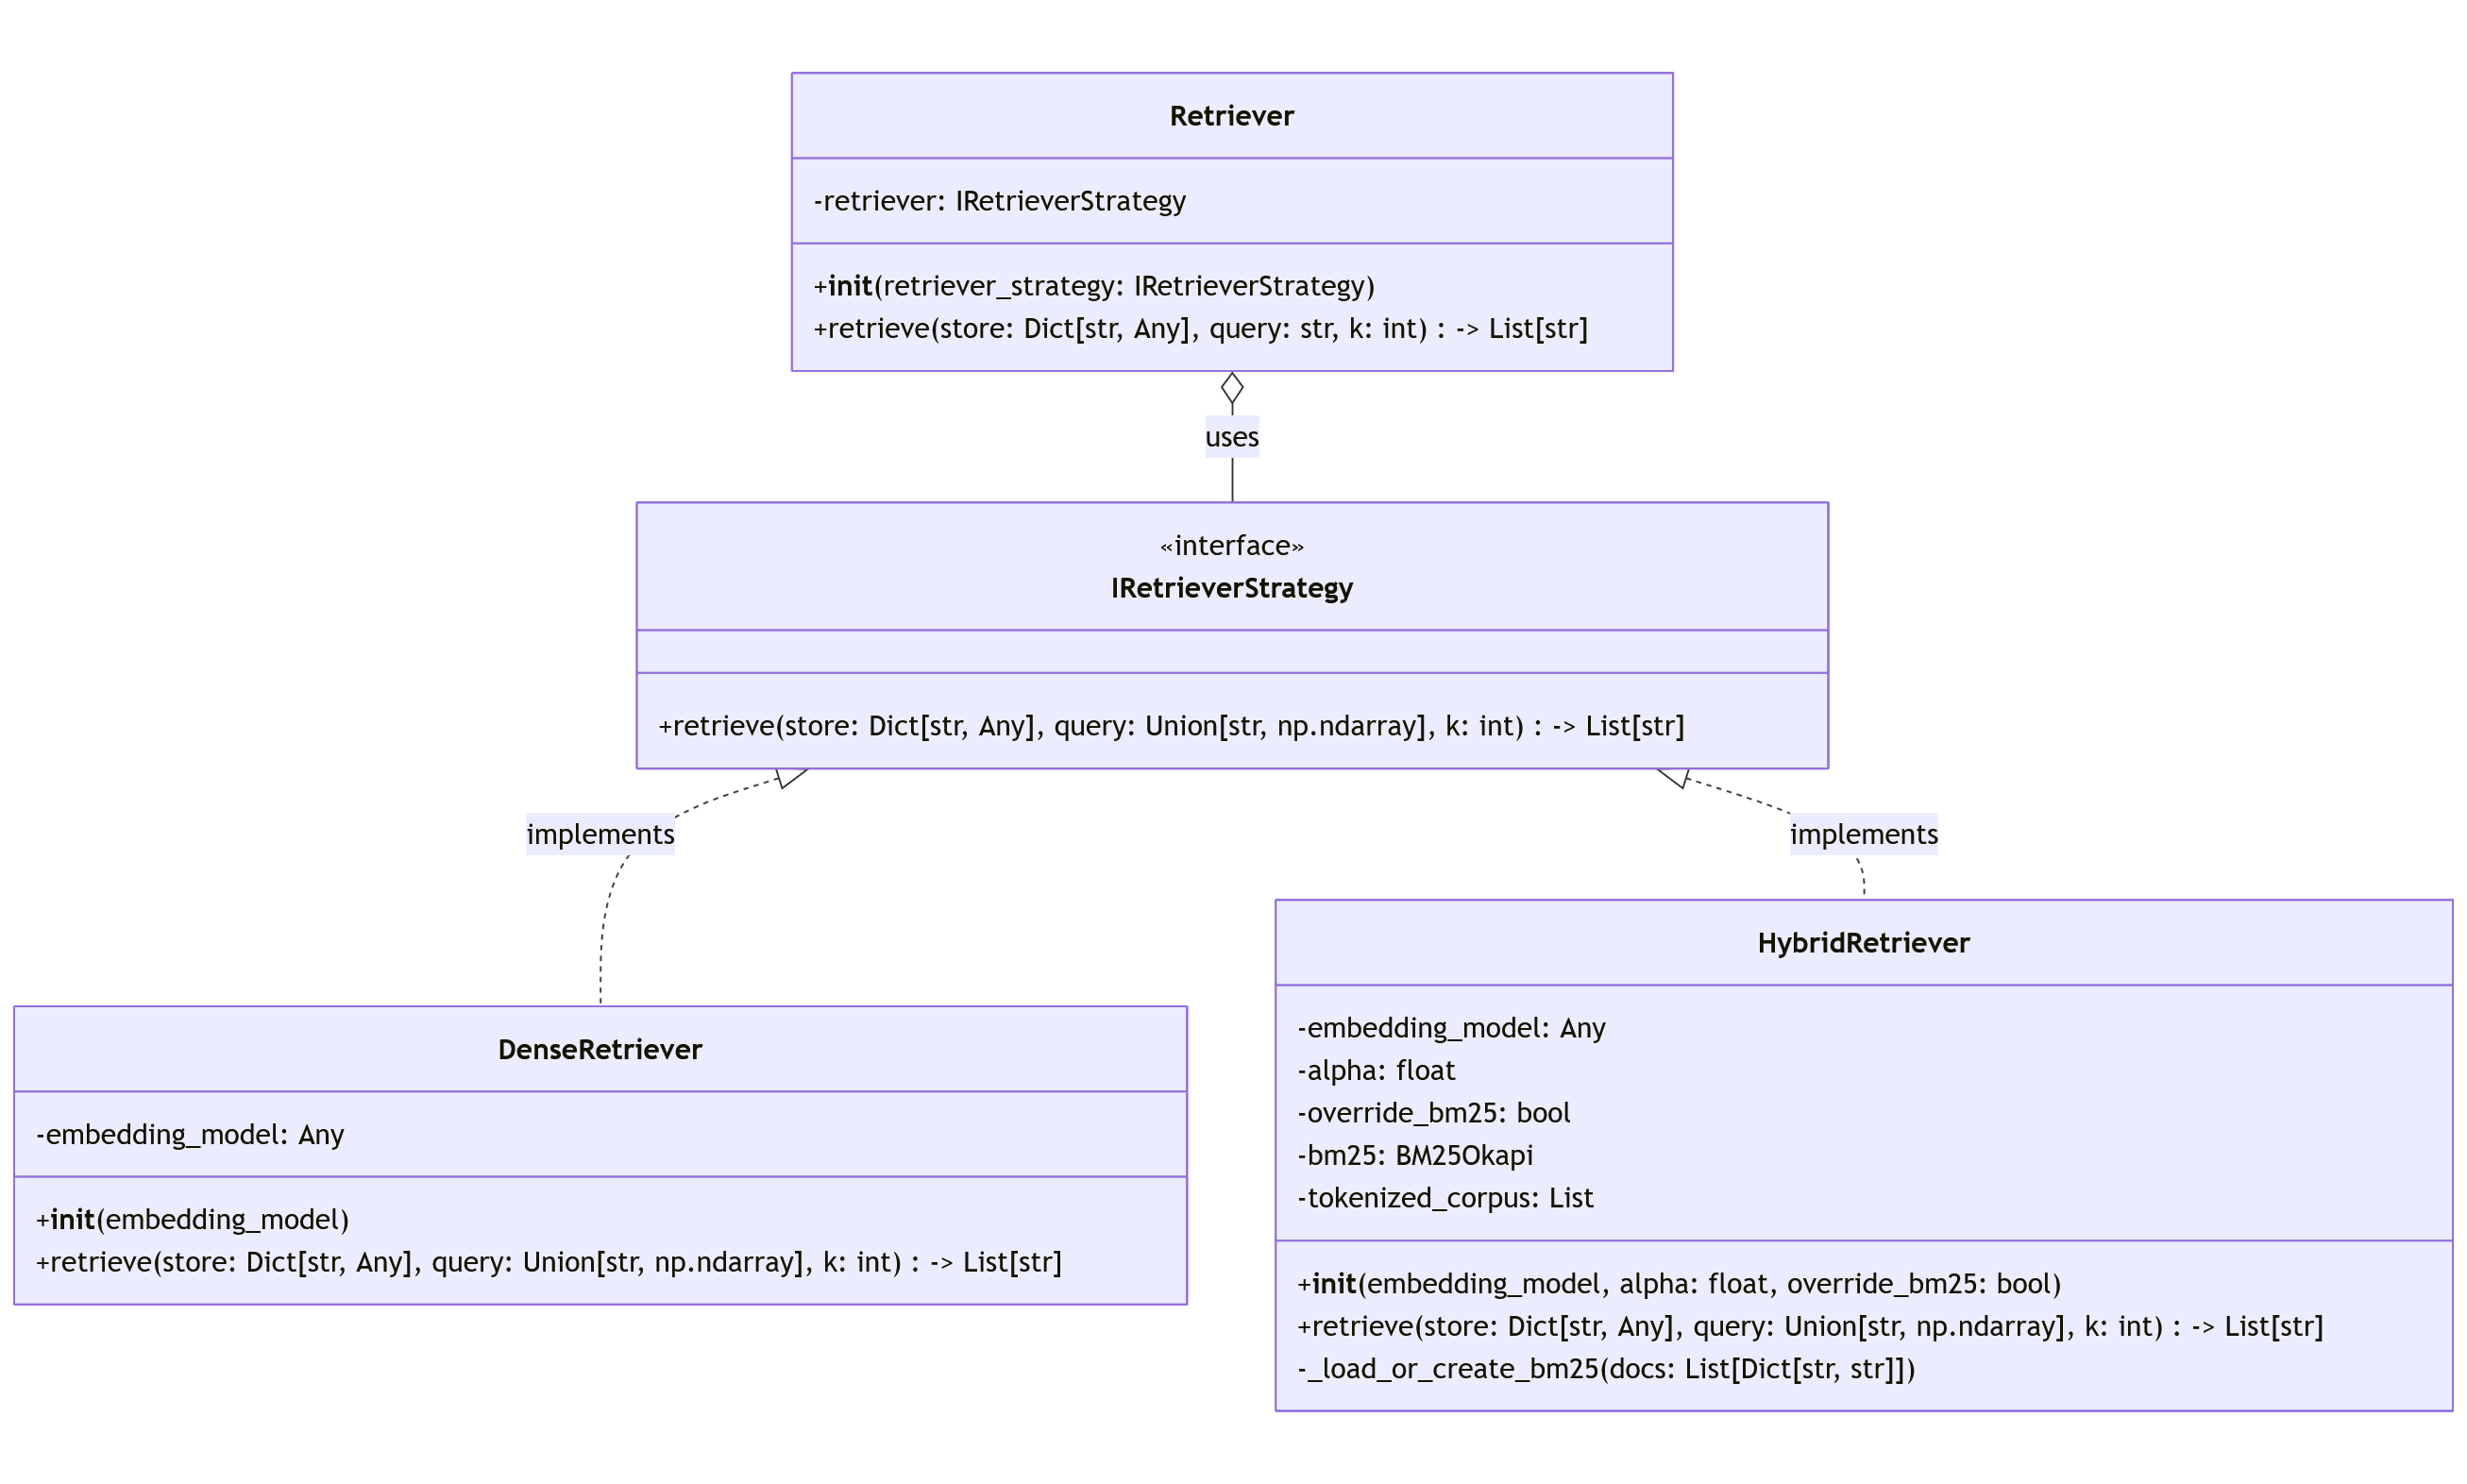
\includegraphics[width=1\linewidth]{img/retriever.png}
    \caption{Diagrama de clase \textit{Retriever}}
    \label{fig:retriever}
\end{figure}


\paragraph{DenseRetriever}

Implementa una estrategia de recuperación basada en similitud de vectores densos generados por modelos de lenguaje.

\begin{itemize}
    \item \textbf{retrieve()}: Recupera los \texttt{k} documentos más similares a una consulta dada, utilizando \textit{embeddings} normalizados y una estructura de índice vectorial.
\end{itemize}

\paragraph{HybridRetriever}

Combina la recuperación densa con un modelo \textit{BM25} de recuperación basada en palabras clave, ponderando ambas con un factor $\alpha$.

\begin{itemize}
    \item \textbf{Constructor}: Inicializa con un modelo de \textit{embeddings}, un valor $\alpha$ para ponderar las dos fuentes de puntuación, y una bandera para sobreescribir el modelo \textit{BM25} guardado.
    \item \textbf{\_load\_or\_create\_bm25()}: Carga un modelo \textit{BM25} desde disco si está disponible o lo crea desde el corpus.
    \item \textbf{retrieve()}: Calcula puntuaciones densas y dispersas, normaliza ambas y las combina según $\alpha$ para recuperar los documentos más relevantes.
\end{itemize}

\subsubsection{VectorDB}

\begin{figure}[htp]
    \centering
    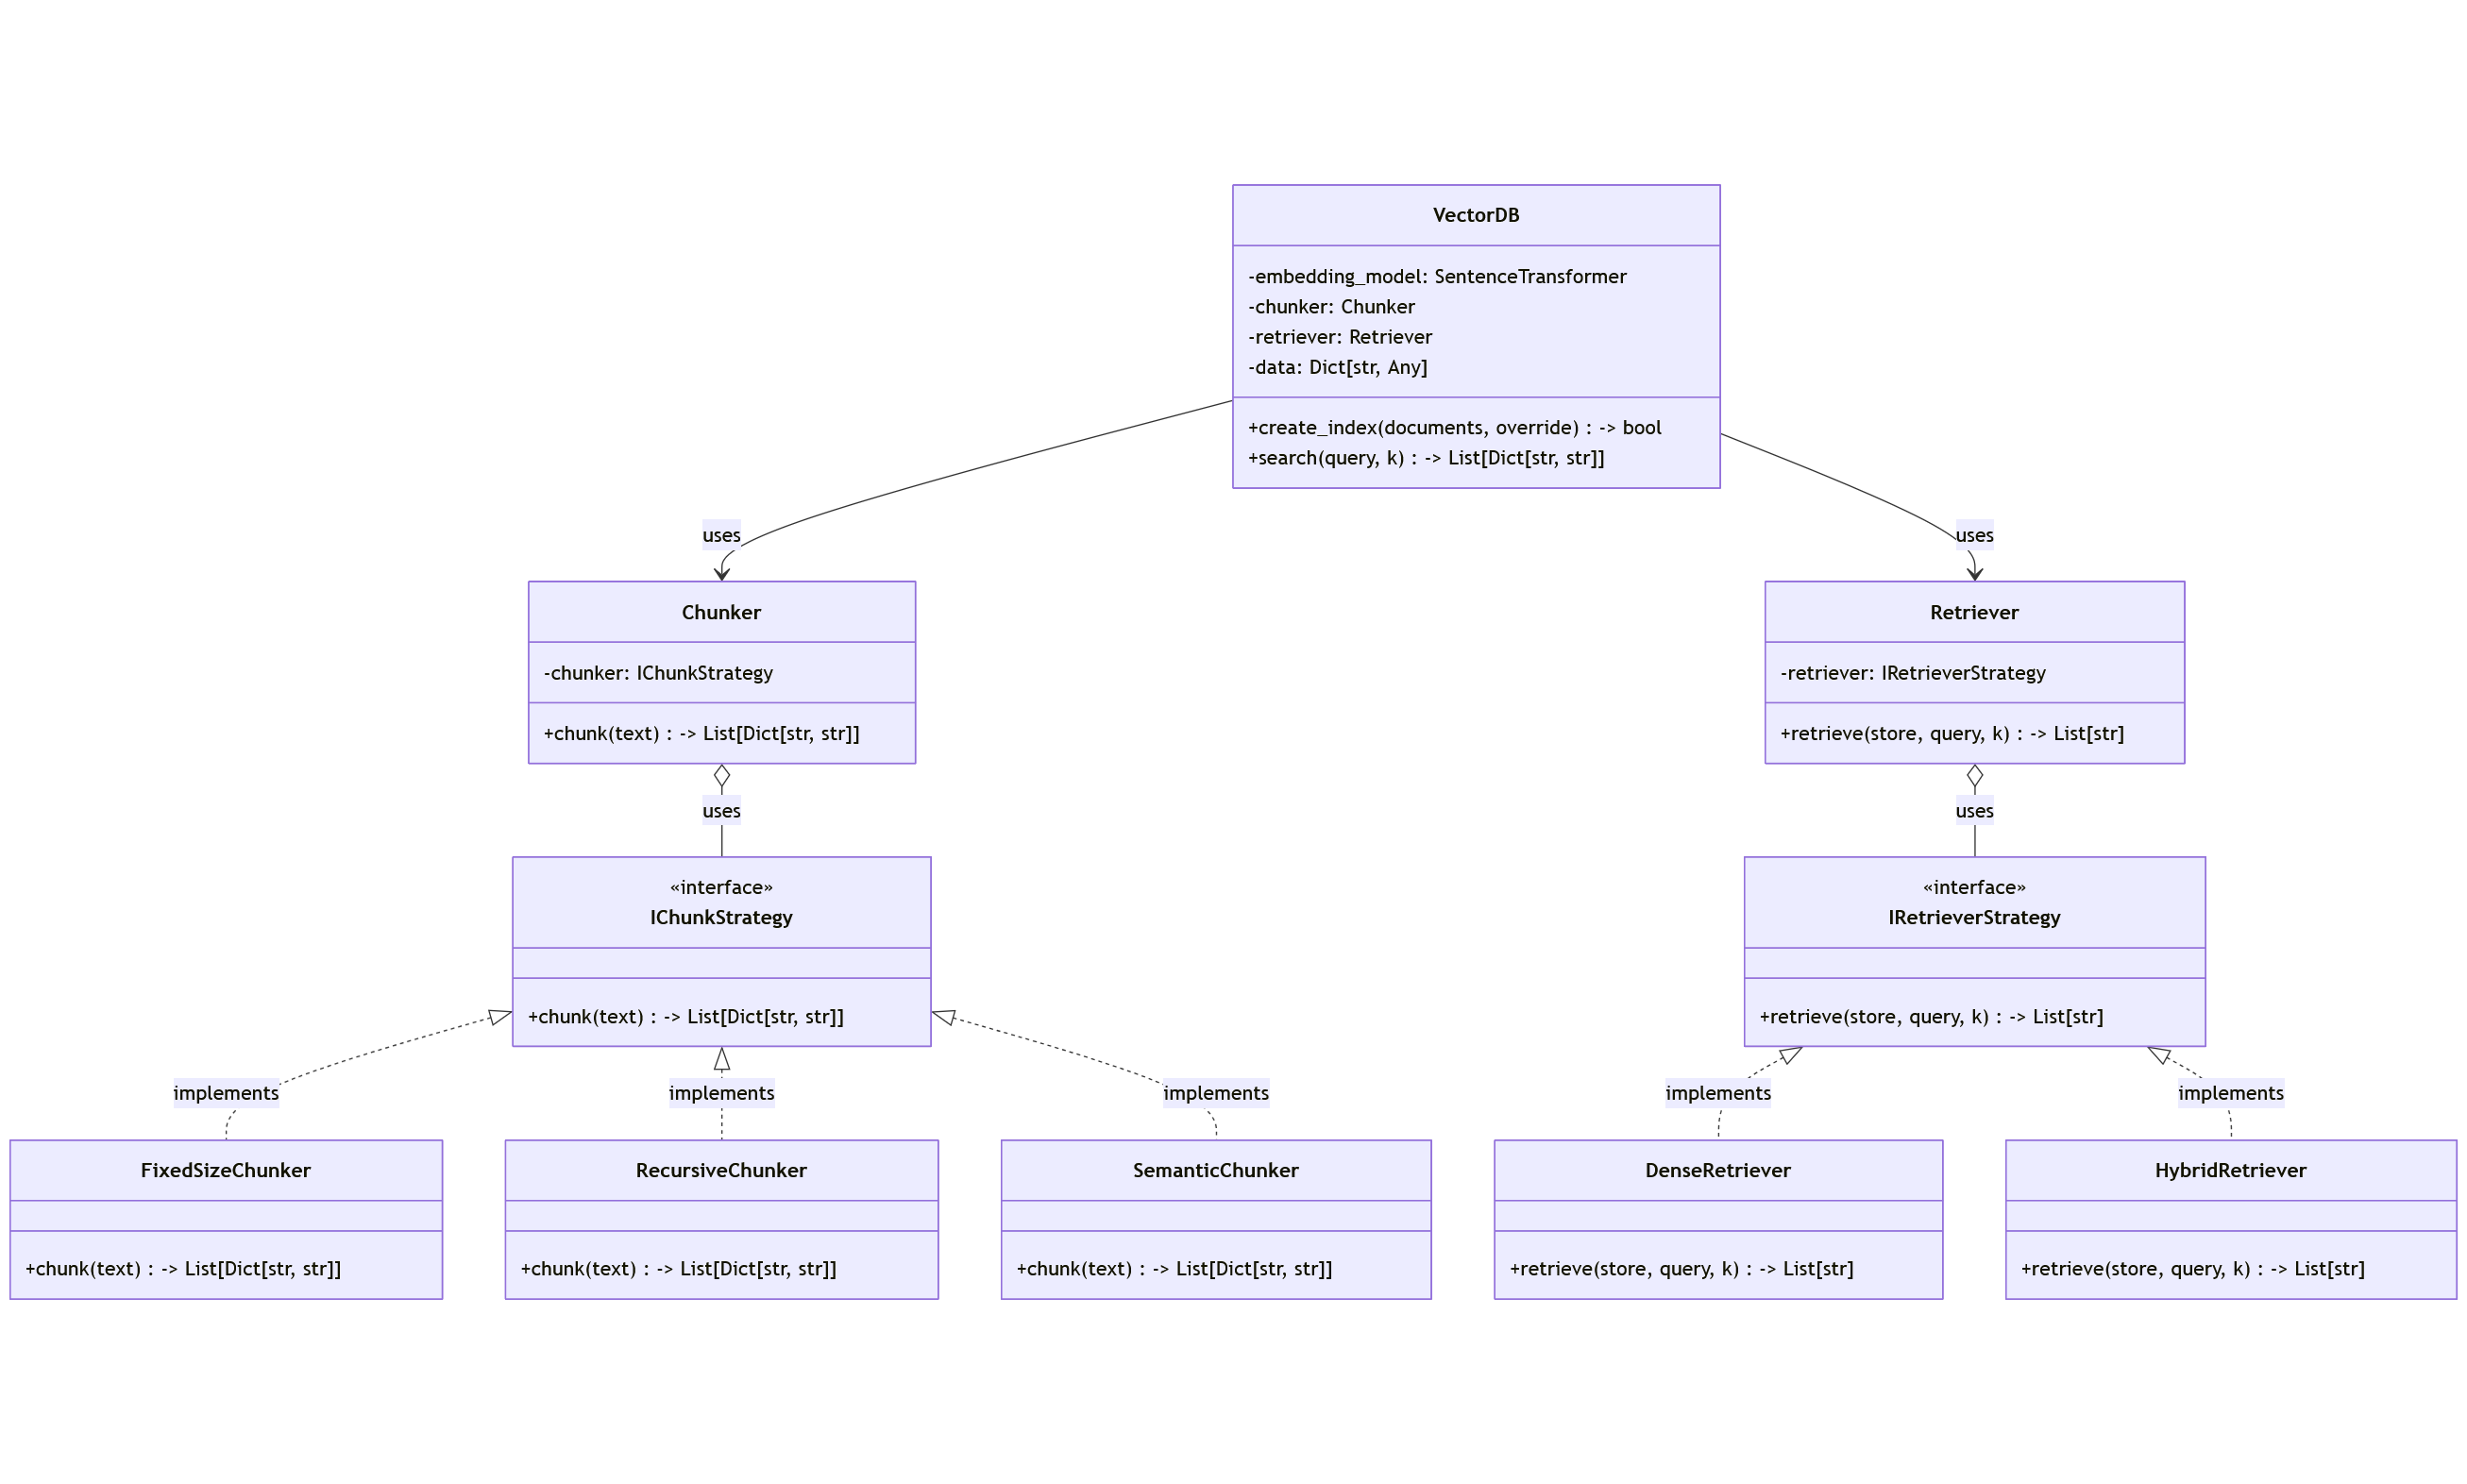
\includegraphics[width=1\linewidth]{img/vectordb.png}
    \caption{Diagrama de clase \textit{VectorDB}}
    \label{fig:vectordb}
\end{figure}

La clase \texttt{VectorDB} implementa una base de datos vectorial que permite gestionar documentos mediante \textit{embeddings} generados con modelos de \texttt{SentenceTransformer}. Esta clase es responsable de la creación de un índice de búsqueda eficiente utilizando \texttt{FAISS} y proporciona métodos para almacenar, cargar y realizar búsquedas sobre los documentos indexados.

\paragraph{Constructor}

El constructor de \texttt{VectorDB} recibe varios parámetros. El primero de ellos es \texttt{embedding\_model}, que puede ser un nombre de modelo o un objeto \texttt{Sentence-Transformer}. Este modelo se utiliza para generar los \textit{embeddings} de los documentos. También recibe un \texttt{chunker}, que es el responsable de dividir los documentos en fragmentos manejables, y un \texttt{retriever}, que se utiliza para la búsqueda de documentos relevantes. Además, se puede especificar la ruta de almacenamiento de los datos con el parámetro \texttt{path}.

\paragraph{Métodos}

\texttt{VectorDB} incluye varios métodos importantes:

\begin{itemize}
    \item \textbf{\_create\_dir(path)}: Este método intenta crear el directorio en la ruta especificada si no existe.
    \item \textbf{\_generate\_embeddings(documents)}: Genera los embeddings para una lista de documentos. Para ello, primero divide los documentos en fragmentos utilizando el \texttt{chunker} y luego calcula los embeddings de cada fragmento.
    \item \textbf{\_save(index, documents)}: Guarda el índice de \texttt{FAISS} y los documentos en la ruta de almacenamiento especificada.
    \item \textbf{\_load()}: Carga los datos previamente almacenados desde un archivo.
    \item \textbf{create\_index(documents, override)}: Crea un índice de \texttt{FAISS} a partir de los embeddings generados. Si el índice ya existe y \texttt{override} es \texttt{False}, simplemente carga el índice existente.
    \item \textbf{search(query, k)}: Realiza una búsqueda de los \texttt{k} documentos más relevantes con respecto a la consulta proporcionada utilizando el \texttt{retriever}.
\end{itemize}

\section{Chatbot}
El agente creado con \textit{LangGraph} utiliza la herramienta del \textit{RAG}, de forma que esta será usada solo cuando convenga al agente. El \textit{workflow} seguido es el que se observa en la figura \ref{fig:flow}

\begin{figure}[htp]
    \centering
    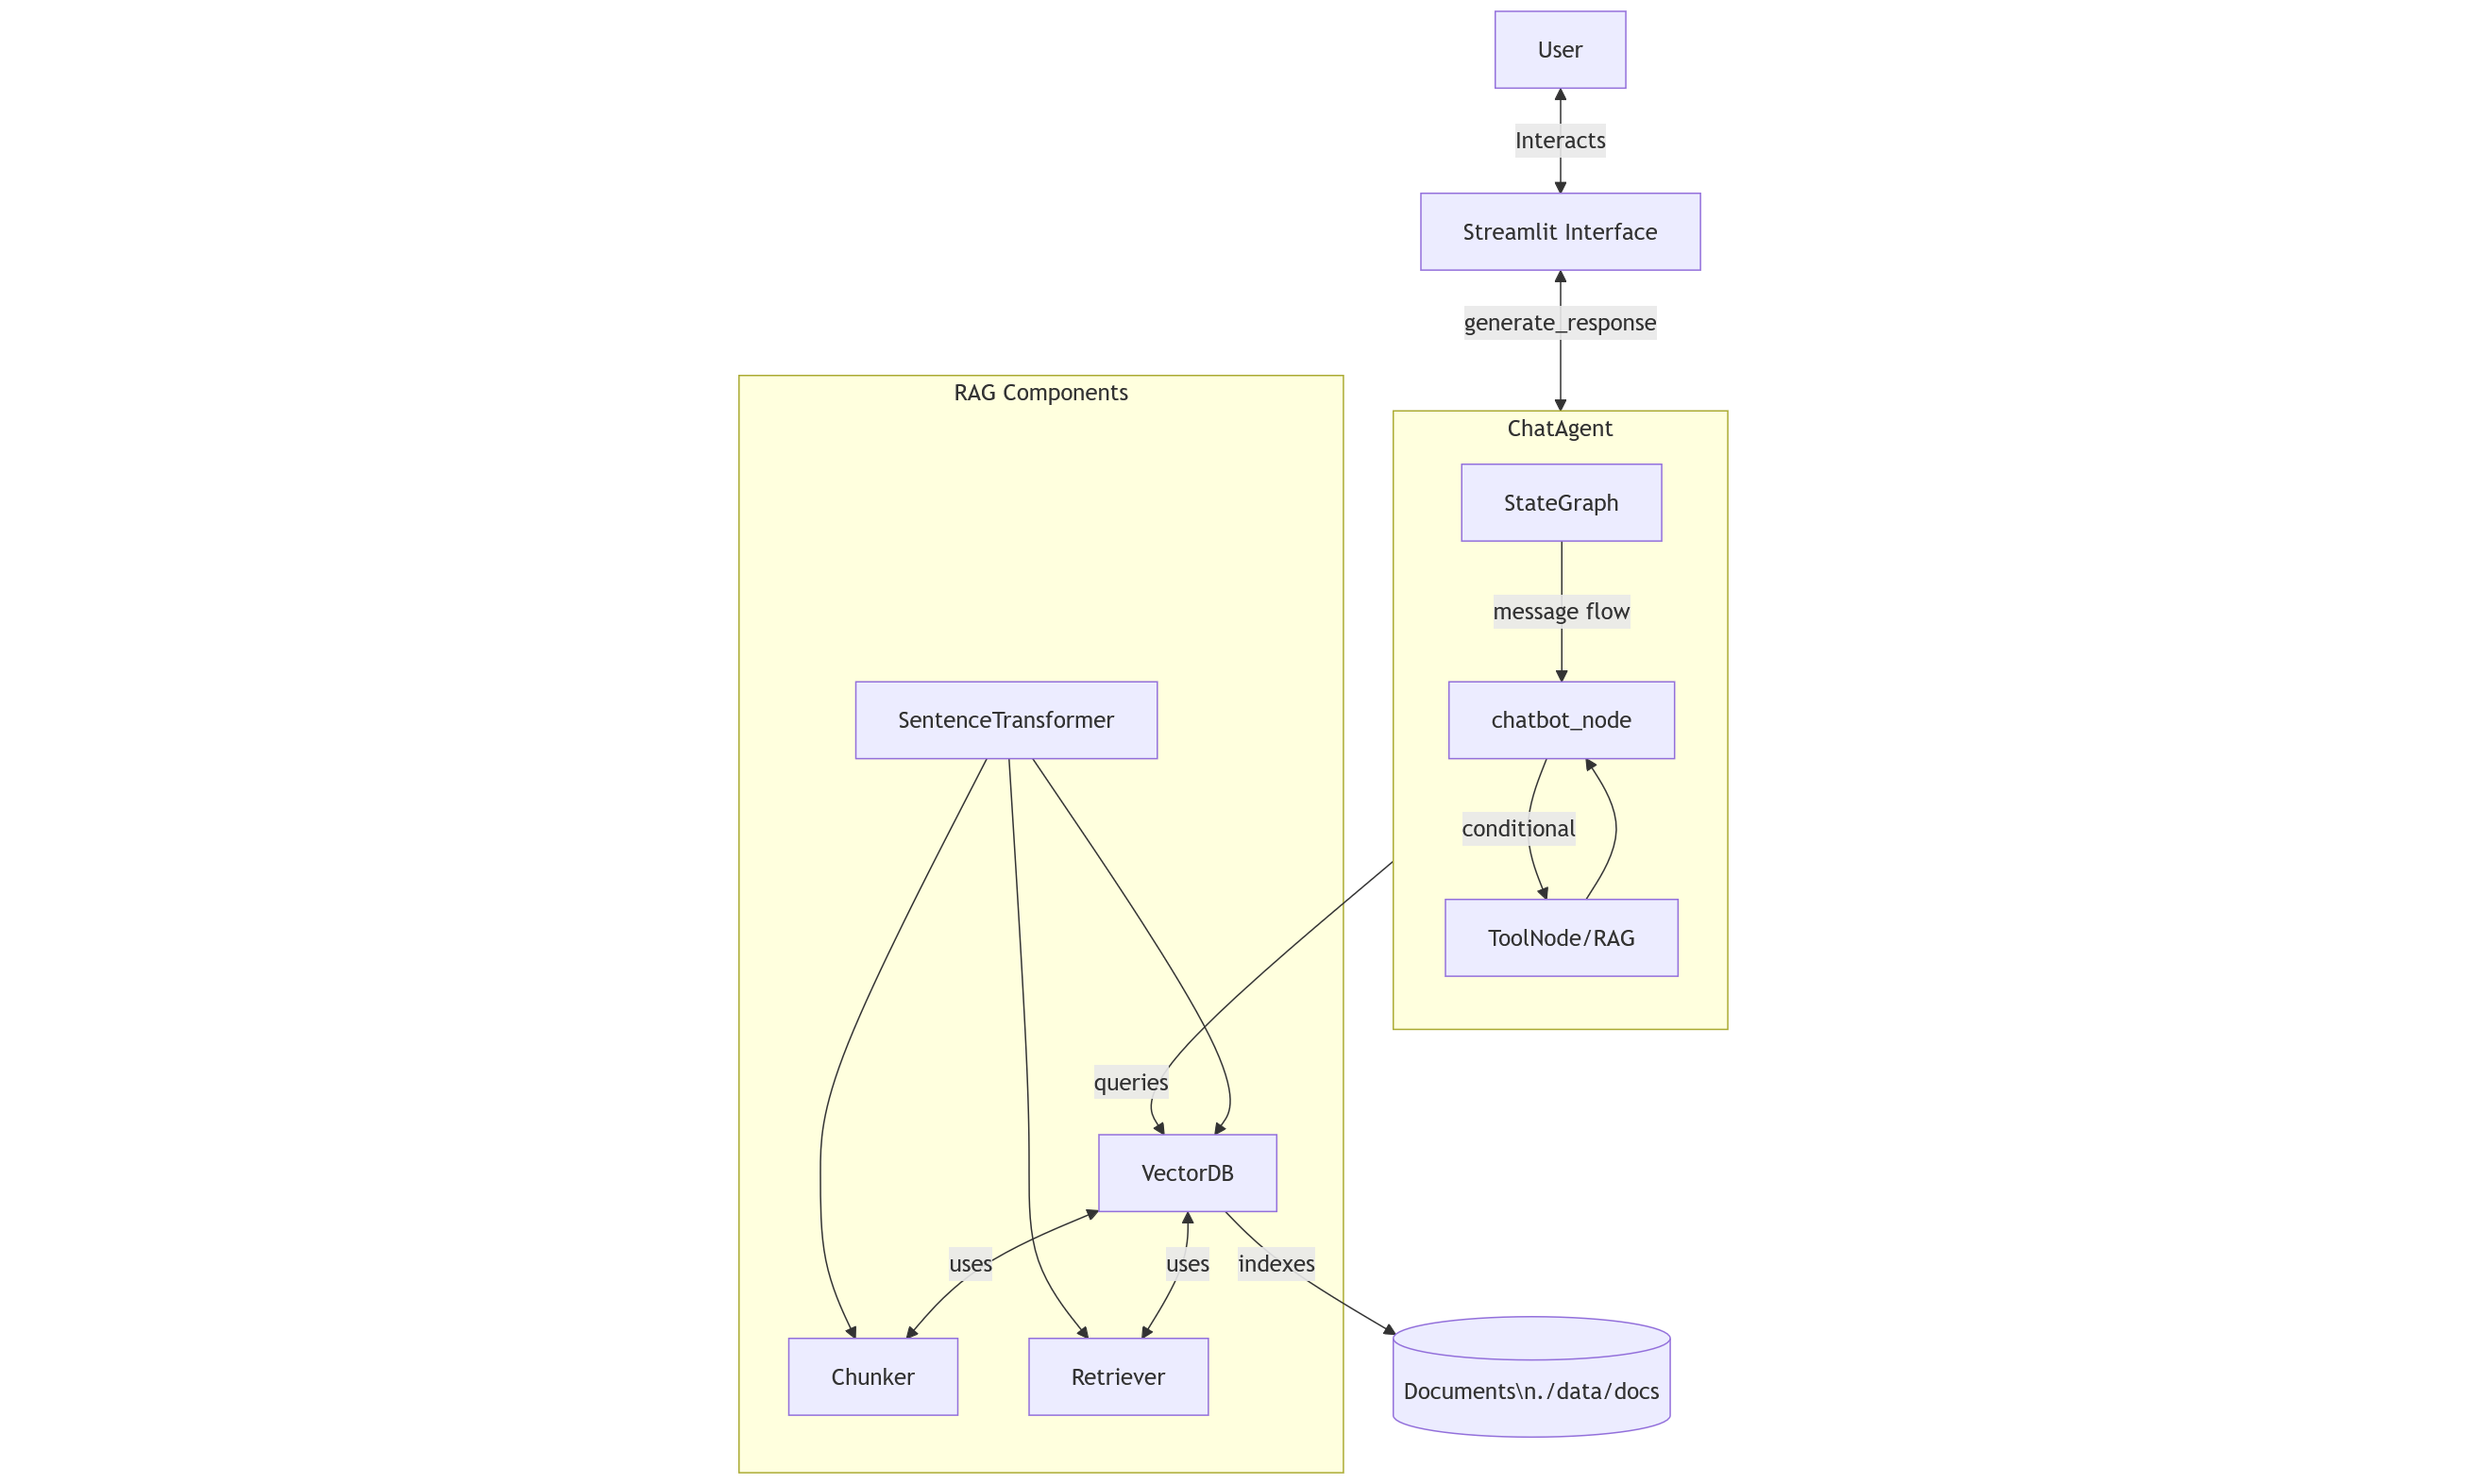
\includegraphics[width=1\linewidth]{img/flow.png}
    \caption{Diagrama de flujo del sistema del agente conversacional con \textit{RAG}}
    \label{fig:flow}
\end{figure}

\subsection{Conversaciones}
Se han utilizado datos de los apuntes generados por el estudiante en formato \textit{Markdown} durante el transcurso de sus estudios en Ingeniería Informática y en el Máster de Ciencia de Datos. El agente tiene instrucciones de usar el \textit{RAG} cuando se le pregunten cosas del ámbito técnico informático.

\begin{figure}[htp]
    \centering
    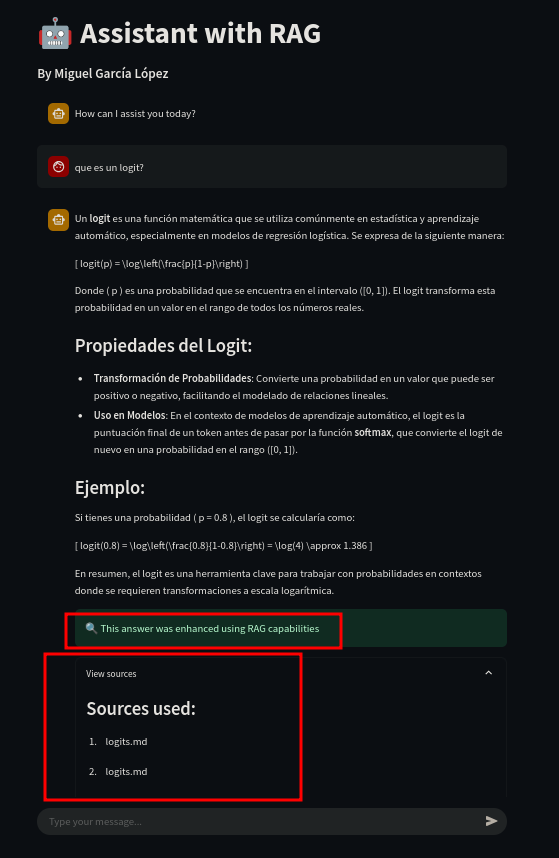
\includegraphics[width=0.7\linewidth]{img/rag-conversation.png}
    \caption{Ejemplo de pregunta técnica en la que se usa el \textit{RAG}}
    \label{fig:rag-conver}
\end{figure}

\newpage
\printbibliography
\end{document}
